\documentclass[spanish, c]{beamer}

\usepackage[utf8]{inputenc}
% \usepackage[spanish, mexico]{babel}
\usepackage{amsmath}
\usepackage{mathtools}
\usepackage{hyperref}
\usepackage{xcolor}
\usepackage{color}
\usepackage{ragged2e}
\usepackage{mathrsfs}
% \usepackage{csquotes}
% \usepackage{listings}
\usepackage[scaled]{beramono}
\usepackage[T1]{fontenc}
\usepackage{graphicx}
\usepackage{booktabs}
\usepackage{physics}
\usepackage{minted}
\usepackage{tcolorbox}
\usepackage{tikz}
\usepackage{relsize}
\usepackage{algorithm}
\usepackage{algpseudocode}

\tcbuselibrary{minted, skins}

\renewcommand{\indent}{\hspace*{2em}}

\newcommand\CC{C\nolinebreak[4]\hspace{-.05em}\raisebox{.4ex}{\relsize{-3}{\textbf{++}}}~}
\newcommand{\bigO}{\mathcal{O}}

\renewcommand{\Comment}[2][.55\linewidth]{%
  \leavevmode\hfill\makebox[#1][l]{\fontfamily{cmss}\selectfont\color{red}\footnotesize$\longrightarrow$\quad#2}}
% \usepackage{tikz}

% \usetikzlibrary{fit, shapes, arrows}

% \usepackage{courier}
% \usepackage{subfigure}
% \usepackage{enumerate}
% \usepackage{algorithmic}
% \usepackage{algorithm}

% \usepackage{listings}
% \usepackage{lstlinebgrd}

\usetheme{Boadilla}
\usefonttheme[onlymath]{serif}

\newcommand\blfootnote[1]{%
\begingroup
\renewcommand\thefootnote{}\footnote{#1}%
\addtocounter{footnote}{-1}%
\endgroup
}

\algrenewcommand\alglinenumber[1]{\footnotesize #1}

\makeatletter
% start with some helper code
% This is the vertical rule that is inserted
\newcommand*{\algrule}[1][\algorithmicindent]{%
  \makebox[#1][l]{%
    \hspace*{.2em}% <------------- This is where the rule starts from
    \vrule height .75\baselineskip depth .25\baselineskip
  }
}

\newcount\ALG@printindent@tempcnta
\def\ALG@printindent{%
    \ifnum \theALG@nested>0% is there anything to print
    \ifx\ALG@text\ALG@x@notext% is this an end group without any text?
    % do nothing
    \else
    \unskip
    % draw a rule for each indent level
    \ALG@printindent@tempcnta=1
    \loop
    \algrule[\csname ALG@ind@\the\ALG@printindent@tempcnta\endcsname]%
    \advance \ALG@printindent@tempcnta 1
    \ifnum \ALG@printindent@tempcnta<\numexpr\theALG@nested+1\relax
    \repeat
    \fi
    \fi
}
% the following line injects our new indent handling code in place of the default spacing
\patchcmd{\ALG@doentity}{\noindent\hskip\ALG@tlm}{\ALG@printindent}{}{\errmessage{failed to patch}}
\patchcmd{\ALG@doentity}{\item[]\nointerlineskip}{}{}{} % no spurious vertical space
% end vertical rule patch for algorithmicx
\makeatother
%

% Sets the templates
\definecolor{navyblue}{RGB}{0, 0, 128}
\definecolor{crimson}{RGB}{128, 16, 0}

\setbeamertemplate{navigation symbols}{}
\setbeamertemplate{headline}{}
\setbeamertemplate{title page}[default][colsep=-4bp,rounded=true]
\setbeamertemplate{footline}[frame number]
\setbeamertemplate{bibliography item}[text]
\setbeamertemplate{theorems}[numbered]

\setbeamercolor{title}{fg=navyblue, bg=white}
\setbeamercolor{frametitle}{fg=navyblue, bg=white}
\setbeamercolor{structure}{fg=navyblue}
\setbeamercolor{button}{fg=white,bg=navyblue}

\setbeamercovered{transparent}

\tcbset{cppexample/.style={%
    colback=green!5,
    colframe=green!30!black,
    listing only,
    fonttitle=\bfseries,
    listing engine=minted,
    minted language=c++,
    minted options={fontsize=\scriptsize, breaklines, linenos, autogobble, numbersep=2mm},
    enhanced,
    overlay={\begin{tcbclipinterior}\fill[red!25!green!25!white] (frame.south west)rectangle ([xshift=4mm]frame.north west);\end{tcbclipinterior}}
}}

\tcbset{cppfullexample/.style={%
    % colback=green!5,
    % colframe=green!30!black,
    listing only,
    fonttitle=\bfseries,
    listing engine=minted,
    minted language=c++,
    minted options={fontsize=\scriptsize, breaklines, linenos, autogobble, numbersep=2mm},
    enhanced,
    overlay={\begin{tcbclipinterior}\fill[black!20!white] (frame.south west)rectangle ([xshift=4mm]frame.north west);\end{tcbclipinterior}}
}}

\tcbset{cppfullborderless/.style={%
    % colback=green!5,
    % colframe=green!30!black,
    listing only,
    listing engine=minted,
    minted language=c++,
    minted options={fontsize=\scriptsize, breaklines, linenos, autogobble, numbersep=2mm},
    enhanced,
    overlay={\begin{tcbclipinterior}\fill[black!20!white] (frame.south west)rectangle ([xshift=4mm]frame.north west);\end{tcbclipinterior}}
}}

\title{Análisis de Algoritmos}
\subtitle{Programación de Estructuras de Datos y Algoritmos Fundamentales \\ (TC1031)}
\author{
    \texorpdfstring{
        \begin{center}
            M.C. Xavier Sánchez Díaz \\
            \href{mailto:sax@tec.mx}{\texttt{sax@tec.mx}}
        \end{center}
    }
    {M.C. Xavier Sánchez Díaz}
}

\institute[Tecnológico de Monterrey]{
\includegraphics[scale=0.5]{../img/logo}}
\date{}

\begin{document}

\setlength{\rightskip}{0pt}

\begin{frame}[plain]
    \titlepage        
\end{frame}

\begin{frame}{Outline}
    \tableofcontents
\end{frame}

\section{Introducción}
\begin{frame}{Algoritmo}{Introducción}
    \begin{center}
        \huge
        ¿Qué es un \textit{algoritmo}?
    \end{center}
\end{frame}

\begin{frame}{Eficiencia de un algoritmo}{Introducción}
    \textbf{Q}: Si tuviéramos dos algoritmos que resuelven el mismo problema\dots ¿cómo sabemos cuál de ellos nos conviene utilizar? \pause

    \bigskip

    \begin{center}
        \textbf{A}: Aquél que sea el más \textit{eficiente} (casi siempre) \pause
    \end{center}

    \bigskip

    Ya sea hablando de \textbf{tiempo de ejecución} o bien en \textbf{uso de espacio en memoria}.\blfootnote{¿Qué es más barato? ¿Tiempo de procesamiento o almacenamiento?}
\end{frame}

\begin{frame}{Tiempo de Ejecución}{Introducción}
El \alert{tiempo de ejecución} de un algoritmo depende de muchos factores: \pause
\bigskip
\begin{enumerate}[<+->]
    \itemsep2ex
    \item {\color<6>{blue}\textbf{Entrada del programa}}. No es lo mismo ordenar una lista con 10 elementos que una de 1 millón de elementos.
    \item \textbf{Calidad del código compilado}. Existen algunas instrucciones más rápidas que otras, y algunos compiladores más veloces que otros.
    \item \textbf{Implicaciones de hardware}. Algunos procesadores son más rápidos que otros.
    \item {\color<6>{blue}\textbf{Complejidad del problema}}. Es más difícil multiplicar dos matrices que ordenar una lista.
\end{enumerate}
\end{frame}

\begin{frame}{Complejidad}{Introducción}
La \alert{complejidad} \textbf{temporal} de un algoritmo hace referencia al tiempo requerido por un algoritmo para ejecutarse, expresado con base en una \textbf{función} que depende del \alert{tamaño} del problema. \pause

\bigskip

Podemos usar la misma idea para expresar también su \textbf{complejidad espacial}, es decir el \textbf{espacio en memoria} que necesita dicho algoritmo\dots
\end{frame}

\begin{frame}{Ejemplo}{Complejidad}

    \begin{algorithmic}[0]
        \State z = 0; \Comment{1 asignación}
        \For {x = 1;  x $\leq n$; x++} \Comment{1 asignación + $(n+1)$ comparaciones}
            \For {y = 1; y $\leq n$; y++} \Comment{$n(n+2) = n^2 + 2n$}
                \State z = z + a[x, y]; \Comment{$n \times n = n^2$}
            \EndFor \Comment{$2n^2$ (incremento + 1 \texttt{goto} implícito)}
        \EndFor \Comment{$n$ (\texttt{goto} implícito cuando y sea \texttt{false})}
        \Statex \Comment{$2n$ (incremento + \texttt{goto} implícito)}
        \Statex \Comment{1 (\texttt{goto} implícito cuando x sea \texttt{false})}
    \end{algorithmic}
    \bigskip
    \begin{center}
        \huge
        Total $ = 4n^2 + 6n + 4$
    \end{center}

\end{frame}

\section{Orden Asintótico}

\begin{frame}{Notación asintótica: $\bigO(g)$}{Orden Asintótico}
    \begin{definition}
        Sea $g \colon \mathbb{N} \to \mathbb{R}^{+}$. $\bigO(g)$ es el conjunto de funciones $f \colon \mathbb{N} \to \mathbb{R}^{+}$ tal que para cualquier constante $c \in R^{+}$ y alguna $n_0 \in \mathbb{N}$, $f(n) \leq cg(n) \forall n \geq n_0$.
    \end{definition}

    \begin{center}
        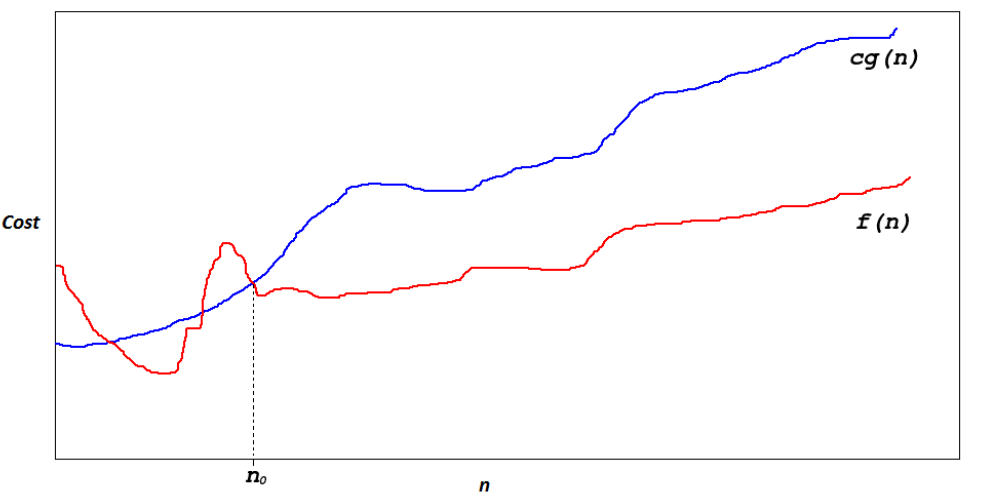
\includegraphics[width=0.85\textwidth]{bigo.png}
    \end{center}
\end{frame}

\begin{frame}{Ejemplos}{Notación asintótica}
    \begin{itemize}
        \itemsep3ex
        \item $g = n +5$ pertenece al grupo de funciones $\bigO(n)$ pues $n+5 \leq 2n$ para cada $n \geq 5$.
        \item $g = (n+1)^2$ es del grupo $\bigO(n^2)$ porque $(n+1)^2 \leq 4n^2$ para cada $n \geq 1$.
        \item $g = n+1)^2$ no es del grupo $\bigO(n)$ porque para cualquier $c > 1$ no se cumplirá nunca que $(n+1)^2 \leq cn$.
    \end{itemize}
\end{frame}

\begin{frame}{Otra manera de verlo}{Orden asintótico}
    Podemos pensar en la notación de $\bigO(g)$  como un ``\textit{a lo mucho}'': \pause
    \bigskip
    \begin{center}
        $g = n + 5$ crece \alert{a lo mucho} como $n$
    \end{center} \pause
    \bigskip
    pues la notación $\bigO$ impone un \textbf{límite superior} (\textit{upper bound}).
\end{frame}

\begin{frame}{Notación asintótica: $\Omega(g)$ y $\Theta(g)$}{Orden asintótico}
    \begin{itemize}
        \itemsep3.5ex
        \item $\Omega(g)$ se usa como un \textbf{límite inferior} (\textit{lower bound}), es decir que una función $f \in \Omega(g)$ es una función que crece \alert{al menos} tan rápido como $g$.
        \item $\Theta(g)$ se usa para definir un grupo de funciones del \textbf{mismo orden}, es decir que una función $f \in \Theta(g)$ es una función que crece \alert{igual} de rápido como $g$.
    \end{itemize}
\end{frame}

\begin{frame}{Órdenes más comunes}{Orden Asintótico}
    \begin{itemize}
        \item $\bigO(1)$ que es constante
        \item $\bigO(\log n)$ que es logarítmico
        \item $\bigO(n)$ que es \textit{lineal}
        \item $\bigO(n \log n)$
        \item $\bigO(n^2)$ que es \textit{cuadrático}
        \item $\bigO(n^2 log n)$
        \item $\bigO(n^m)$ que es \textit{polinomial}
        \item $\bigO(m^n)$ que es \textit{exponencial}
        \item $\bigO(n!)$ que es \textit{factorial}
    \end{itemize}
\end{frame}

\section{Análisis Práctico}

\begin{frame}{Reglas de dedo para análisis de algoritmos}{Análisis Práctico}

    El uso del \textbf{orden asintótico} nos ayuda a simplificar el análisis de complejidad de los algoritmos. \pause

    \bigskip

    Para hacerlo más \textit{sencillo}, lo que suele hacerse es usar la notación de $\bigO$ debido a que es la que agrega un \textbf{límite superior}, quitando coeficientes y quedándonos con alguno de los órdenes comunes: \pause

    \bigskip

    \begin{center}
        \huge
        \textit{En el peor de los casos, este algoritmo será, a lo mucho, igual de tardado que este otro}
    \end{center}
\end{frame}

\begin{frame}{Instrucciones secuenciales}{Análisis Práctico}
    
    \begin{columns}
        \begin{column}{0.35\textwidth}
            \begin{center}
                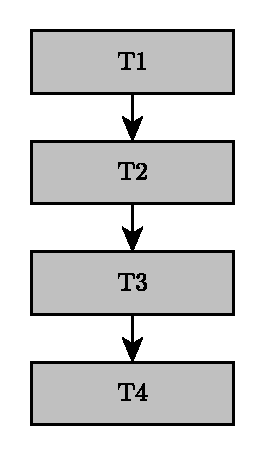
\includegraphics[width=0.75\textwidth]{sequential-times.pdf}
            \end{center}
        \end{column}
        \begin{column}{0.65\textwidth}
            \hspace{-1in}
            \begin{itemize}
                \item \textbf{Complejidad exacta}: $\Theta(\sum T_i)$
                \item \textbf{Complejidad asintótica}: $\bigO(\max(T_i))$
            \end{itemize}

            \bigskip

            Por ejemplo, una secuencia de 4 instrucciones donde:
            \begin{itemize}
                \item $T_1 = \bigO(n)$
                \item $T_2 = \bigO(\log n)$
                \item $T_3 = \alert{\bigO(n^2)}$
                \item $T_4 = \alert{\Theta(2n^2 + 3)}$
            \end{itemize}

            \bigskip

            tendrá entonces una complejidad de $T = \alert{\bigO(n^2)}$
        \end{column}
    \end{columns}
\end{frame}

\begin{frame}{Decisiones}{Análisis Práctico}
    
    \begin{columns}
        \begin{column}{0.35\textwidth}
            \begin{center}
                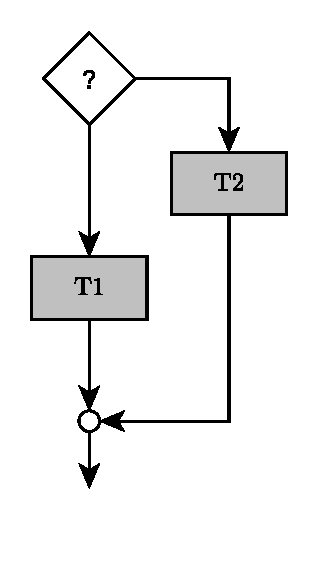
\includegraphics[width=0.85\textwidth]{decision-times.pdf}
            \end{center}
        \end{column}
        \begin{column}{0.65\textwidth}
            \hspace{-1in}
            \begin{itemize}
                \item \textbf{Complejidad promedio}: $\text{avg} (T_1, T_2)$
                \item \textbf{Complejidad asintótica}: $\bigO(\max(T_1, T_2))$
            \end{itemize}

            \bigskip

            Por ejemplo, una decisión con 2 ramas de instrucciones donde:

            \begin{itemize}
                \item $T_1 = \bigO(\log n)$
                \item $T_2 = \alert{\bigO(n \log n)}$
            \end{itemize}

            \bigskip

            tendrá entonces una complejidad de $T = \alert{\bigO(n \log n)}$
        \end{column}
    \end{columns}
\end{frame}

\begin{frame}{Ciclos}{Análisis Práctico}
    
    \begin{columns}
        \begin{column}{0.35\textwidth}
            \begin{center}
                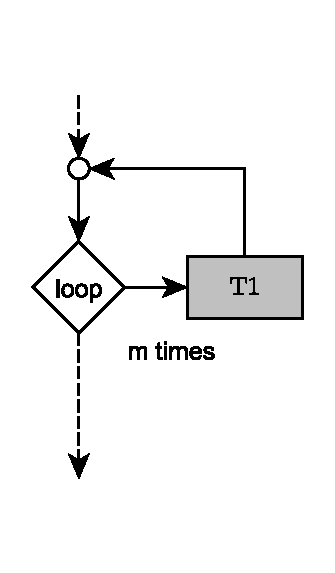
\includegraphics[width=0.95\textwidth]{loop-times.pdf}
            \end{center}
        \end{column}
        \begin{column}{0.65\textwidth}
            \hspace{-1in}
            \begin{itemize}
                \item \textbf{Complejidad exacta}: $\Theta(m T_1)$
                \item \textbf{Complejidad asintótica}: \alert{depende}
            \end{itemize}

            \bigskip

            Por ejemplo, asumiendo que $T_1 = \Theta(n)$:
            
            \begin{itemize}
                \item Si $m << n$ entonces $T = \alert{\bigO(n)}$
                \item Si $m \approx n$ entonces $T = \alert{\bigO(n^2)}$
            \end{itemize}

            Es muy importante considerar que la notación $\bigO$ elimina coeficientes, por lo que a veces no podemos ignorar el tamaño de $m$ si $m \not \ll n$.
        \end{column}
    \end{columns}
\end{frame}

\section{Análisis de algoritmos recursivos}

\begin{frame}{Divide \& Conquer}{Análisis de algoritmos recursivos}

    En el estudio de algoritmos, \alert{divide and conquer} hace referencia a una técnica de diseño que se enfoca en \textbf{partir} un problema en \textbf{problemas más pequeños}: \pause

    \bigskip

    \begin{itemize}[<+->]
        \itemsep2.5ex
        \item La idea es juntar las soluciones de cada \textit{subproblema} y obtener así la solución total del problema original
        \item Esta técnica es muy eficiente cuando se utiliza \textbf{recursión}
        \item La implementación de algoritmos diseñados con esta técnica es ideal para resolverse de manera \textit{paralela}
    \end{itemize}
\end{frame}

\begin{frame}{Máximo y mínimo de un conjunto}{Análisis de algoritmos recursivos}

    \begin{center}
        \huge
        ¿Cuál es la primera idea que viene a tu mente si queremos obtener tanto el máximo como el mínimo de un conjunto?
    \end{center}
    
\end{frame}

\begin{frame}{Análisis del enfoque de Divide \& Conquer}{Análisis de algoritmos recursivos}
    Con una entrada de $n = 2^k$, y considerando que cada \textit{vuelta} \textbf{divides en 2 partes de la mitad del tamaño}, y que en cada vuelta haces \textbf{una} comparación entre \textbf{dos elementos}, entonces: \pause
    \begin{align*}
        T(n) & = 2T\left(\frac{n}{2}\right) + 2  & \tag{$k = 1$}\\ \pause
             & = 2\left(T\left(\frac{\frac{n}{2}}{2}\right) + 2\right) + 2  & \tag{$k = 2$}\\ \pause
             & = 4T\left(\frac{n}{4}\right) + 4 + 2 & \tag{\text{desarrollando}} \\ \pause
             & = 2^2 T\left(\frac{n}{2^2}\right) + 2^2 + 2^1 & \tag{\text{sustituye por }$2^i$} \\ \pause
             & = 2\left(2^2 T\left(\frac{\frac{n}{2^2}}{2}\right) + 2^2  + 2 \right) + 2 & \tag{$k = 3$} \\ \pause
             & = 2^3 T\left(\frac{n}{2^3}\right) + 2^3 + 2^2 + 2 & \tag{\text{desarrolla \& sustituye}} %partir aquí
    \end{align*}
\end{frame}

\begin{frame}{Análisis del enfoque de Divide \& Conquer}{Análisis de algoritmos recursivos}
    \begin{align*}
        & = 2^3 T\left(\frac{n}{2^3}\right) + 2^3 + 2^2 + 2 & \tag{\text{cont.}} \\ 
        & \vdots \\
        & = 2^{k-1} T\left(\frac{n}{2^{k-1}}\right) + {\color{blue} 2^{k-1} + 2^{k-2} + \dots + 2^2 + 2^1} & \tag{\text{tras } $k-1$ \text{ pasos}}
    \end{align*}

    Y considerando que $n = 2^k$, sabemos que $2^{k-1} = \frac{n}{2}$ así que podemos sustituirlo en la ecuación.    
    Del mismo modo, podemos sustituir la parte en {\color{blue} azul} por la sumatoria
    $$\color{blue} \sum\limits_{i=0}^n x^i = \frac{x^{n+1} - 1}{x - 1}$$
    donde $x = 2$ y $n = k-1$. Es importante notar que la sumatoria va desde $0$ hasta $n$. 
    En nuestro caso, empezamos desde $k=1$ en adelante, por lo que hay que restarle el primer término: $2^0 = 1$.
\end{frame}

\begin{frame}{Análisis del enfoque de Divide \& Conquer}{Análisis de algoritmos recursivos}
    Reemplazando entonces la sumatoria, $n$ por $2^k$, tenemos

    \begin{align*}
    & = 2^{k-1} T\left(\frac{2^k}{2^{k-1}}\right) + {\color{blue} \frac{2^k - 1}{2 - 1} - 1} & \tag{\text{sust.}} \\[1.5ex]
    & = \frac{n}{2}T(2) + \frac{n - 1}{1} - 1 & \tag{\text{sust.}} \\[1.5ex]
    & = \frac{n}{2}(1) + n - 2 & \tag{sust.} \\[1.5ex]
    & = \frac{n}{2} + {\color{red} n} - 2
    \end{align*}

    $$\quad \therefore \quad T(n) = {\color{red}\bigO(n)}$$

\end{frame}

\begin{frame}[plain]
    \begin{center}
        \Huge
        Es un show.
    \end{center}
\end{frame}

\begin{frame}{Teorema Maestro}{Análisis de algoritmos recursivos}
    Existe una manera más sencilla de darse cuenta desde el principio dado el tipo de recurrencia.
    
    \bigskip

    Supongamos que $n = c^k$ y $c > 1$. Entonces
    $$T(n) = \begin{cases}
        b & \text{si } n = 1 \\
        aT\left( \frac{n}{c} \right) + bn^x & \text{si } n > 1
    \end{cases}$$

    \begin{itemize}
        \item $a$ es el \alert{número} de \textbf{subproblemas}
        \item $\frac{n}{c}$ es el \alert{tamaño} de los \textbf{subproblemas}
        \item $bn^x$ es el costo de la \alert{operación} realizada en \alert{cada vuelta} (como partir o unir, comparar, sumar, multiplicar\dots)
    \end{itemize}
\end{frame}

\begin{frame}{Teorema Maestro}{Análisis de algoritmos recursivos}
    \begin{theorem}
        Sabiendo que $n = c^k$ y $c > 1$, y 
        $$T(n) =
        \begin{cases}
            b & \text{si } n = 1 \\
            aT\left( \frac{n}{c} \right) + bn^x & \text{si } n > 1
        \end{cases}$$
        entonces
        $$T(n) =
        \begin{cases}
            \Theta (n^{\log_c a}) & \text{si } a > c^x \\
            \Theta (n^x \log_c n) & \text{si } a = c^x \\
            \Theta (n^x) & \text{si } a < c^x
        \end{cases} $$
    \end{theorem}
\end{frame}

\begin{frame}{Propiedades de Logaritmos}{Equivalencias útiles}
    \begin{enumerate}
        \itemsep2.5ex
        \item $\log_b 1 = 0$
        \item $\log_b b^a = a$
        \item $\log_b xy = \log_b x + \log_b y$
        \item $\log_b \dfrac{x}{y} = \log_b x - \log_b y$
        \item $\log_b x^a = a \log_b x$
        \item $x^{\log_b y} = y^{\log_b x}$
        \item $\log_c x = \dfrac{\log_b x}{\log_b c} = (\log_c x)(\log_b c)$
    \end{enumerate}
\end{frame}

\begin{frame}{Equivalencias en sumatorias y series}{Equivalencias}
    \begin{enumerate}
        \item $\displaystyle \sum_{i = 1}^n 1 = n$
        \item $\displaystyle \sum_{i = 1}^n i = \frac{n(n+1)}{2}$
        \item $\displaystyle \sum_{i=0}^n x^i = \frac{x^{n+1} - 1}{x - 1}$
        \item $\displaystyle \sum_{i=1}^n \frac{1}{i} = \ln n$
        \item $\displaystyle \sum_{i=1}^n ix^i = \frac{(n-1)x^{n+1} - nx^n + x}{(x-1)^2}$
        \item $\displaystyle \sum_{i=1}^n i^2 = \frac{n(n+1)(2n + 1)}{6}$
    \end{enumerate}

\end{frame}

% \section*{Referencias}

% \begin{frame}[t]{Referencias}
    % \nocite{bibID01}
    % \nocite{bibID02}

    % \bibliographystyle{IEEE}
    % \bibliography{biblio}
% \end{frame}

\end{document}